\section{Diseño Detallado del Husillo}
Para el diseño y selección de los elementos del subsistema motor-husillo se tiene en cuenta la arquitectura paralela de la herramienta, potencia requerida, velocidades y pares necesarios para la operación de fresado. El subsistema del motor-husillo esto compuesto un motor, una caja de trasmisión y un eje flexible.

\subsection{Selección del motor-husillo}
Para la selección del motor se toma la potencia de corte, velocidad y par que requiere la operación de fresado. La potencia de corte ($P_{c}$) se multiplica por un factor de servicio ($Fs$) y con esta potencia requerida se procede a seleccionar el tipo de motor y posteriormente el motor que se requiere para la operación de fresado.

\begin{equation}
P_{s}=Fs\times P_{c}=1.1kW\times1.3=1.5 kW
\end{equation}

Para la selección de tipo de motores se entra la figura \ref{fig:Seleccion_M} donde se concluye que el tipo de motor que ofrece las mejores prestaciones para el fresado es el motor eléctrico. El motor eléctrico posee las siguientes ventajas frente a los motores neumáticos e hidráulico como los es la precisión, silencioso, factibles y fáciles de controlar.

\begin{figure}[ht]
    \centering
    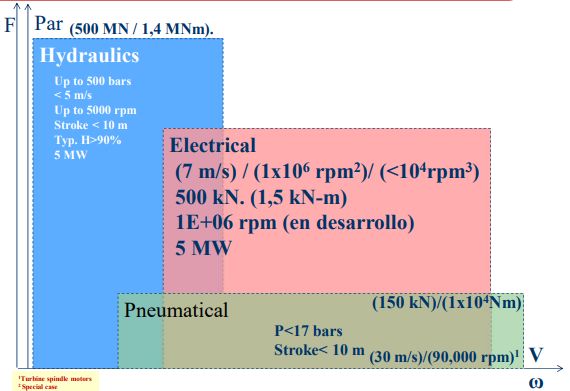
\includegraphics[width =0.9\textwidth]{Cap5_DisenoDetallado/Figuras/Seleccion_M.PNG}
    \caption{Rendimiento cualitativo de los motores}{Fuente: Heriberto Maury}
    \label{fig:Seleccion_M}
\end{figure}

Después de hacer una búsqueda del motor que cumpla las necesidades de la operación de mecanizado. Se encuentra un Spindle servo motor modelo $MK08-3-9.5-1.5/2.2-4-1500$, Este motor trabaja con 3 fases alternas siendo estos motores asíncronos con excelentes características dinámicas. Según \cite{{catalogue:Shenzhen_Guanhong_Technology}} este motor AC asíncrono es normalmente usado en robot, petróleo, metalurgia, equipos de control automático, etc. Las características de este motor se presentan en la tabla \ref{table:Caracteriticas_motor}.

\begin{longtable}{|c|c|c|c|c|c|c|}
\hline
\rowcolor[HTML]{EFEFEF} 
\multicolumn{7}{|c|}{\cellcolor[HTML]{EFEFEF}Moder motor :MK08-3-9.5-1.5/2.2-4-1500}                                                                                                                                                                                                                                                                                                                                                                                                      \\ \hline
\rowcolor[HTML]{EFEFEF} 
\begin{tabular}[c]{@{}c@{}}Reted power\\     (kw)\end{tabular} & \begin{tabular}[c]{@{}c@{}}Rated torque\\     (Nm)\end{tabular} & \begin{tabular}[c]{@{}c@{}}Rated\\   current\\     (A)\end{tabular} & \begin{tabular}[c]{@{}c@{}}Rated speed\\     (rpm)\end{tabular} & \begin{tabular}[c]{@{}c@{}}Max speed\\     (rpm)\end{tabular} & \begin{tabular}[c]{@{}c@{}}Rotor inertia\\     (kg.m\textasciicircum{}2)\end{tabular} & \begin{tabular}[c]{@{}c@{}}weigth\\  (kg)\end{tabular} \\ \hline
1.5                                                            & 9.5                                                             & 3.7                                                                 & 1500                                                            & 8000                                                          & 0.0058                                                                                & 25                                                     \\ \hline

\caption{Caracteristicas del motor}{Fuente:\cite{catalogue:Shenzhen_Guanhong_Technology}}
\label{table:Caracteriticas_motor}
\end{longtable}
\newpage
\subsection{Diseño sistema de transmisión}
La caja de transmisión la cual se requiere para la operación de la máquina debe ser de relación de transmisión variable, por lo cual debe constar con un selector de engranaje el cual permitirá dar diferentes velocidades de salida con un mismo motor.

Para el diseño de la caja de transmisión se trabajará con engranajes helicoidales, los cuales permiten un trabajo a altas velocidades, proveen una alta relación de contacto y además producen bajos niveles de ruido.

Se diseñarán los engranajes según las recomendaciones de la AGMA, se tomarán como base el número de dientes establecidos en el diseño básico y se iniciara un proceso iterativo el cual permita un diseño sin modos de falla, para iniciar el proceso se establecen los ángulos de hélice y de presión de 20° acorde las recomendaciones de diseño y se evalúan modos de fallas cinemáticos y cinéticos. 

Para el diseño Cinemático se tuvieron en cuenta los siguientes modos de fallas:
\begin{itemize}\nosep
    \item  Intermitencia
    \item Interferencia
    \item Ruido
\end{itemize}
Mientras que el diseño cinético se tuvo en cuenta los siguientes modos de falla:
\begin{itemize}\nosep
    \item  Fatiga flexional
    \item Fatiga superficial
\end{itemize}
Para la demostración del diseño se procede a diseñar el engranaje $N° 1$ el cual se encuentra en una relación transmisión de 1, se inicia el proceso de diseño con el diseño cinemático.    

\subsection*{Diseño cinemático}
\subsubsection*{Intermitencia}
Para iniciar el análisis se procede a calcular valores geométricos que se necesitaran para la evaluación del engranaje. 

\begin{equation}
 \phi_{t}=\arctan{\frac{\tan{\phi_{n}}}{\cos{\psi}}}
\label{Eq:1}    
\end{equation}
Donde:\\
$ \phi_{t}$=Ángulo de presión transversal.\\
$\phi_{n}$=Ángulo de presión normal.\\
$\psi$=Ángulo de hélice.

%revisar con jairo
$\phi_t = 21.1728$, $m=2.5$,    Ancho de caro, $F = 12\times m = 30~mm$, paso normal, $P_n=\pi \times m$, donde m es el modulo.
%%%%%
Para la evaluación de intermitencia se calcula un ancho de cara mínimo para el engranaje, este se calcula con la ecuación \ref{Eq:2} de la AGMA Tomada  del \citep{shigley2011shigley}.
\begin{equation}
 F_{min}=b_{min}=\frac{1.15 P_{n}}{\tan{\psi}}
 F_{min}= 24.8154 mm
\label{Eq:2}    
\end{equation}


Con un ancho de cara mayor a un ancho de cara mínimo, se descarta el modo de falla de intermitencia.
\subsubsection*{Interferencia}
La interferencia en los engranajes helicoidales va relacionada con el numero de dientes, un numero de dientes muy pequeño, podría causar un problema de interferencia, por la cual se procede a calcular el número de dientes mínimo  \ref{Eq:3}, para evitar este modo de falla.
\begin{equation}
 N_{p,min}=\frac{2K \cos{\psi}(i+\sqrt{i^{2}+(1+2i\sin{\phi_{t}}^{2})}}{(1+2i)\sin{\phi_{t}}^{2}}
\label{Eq:3}    
\end{equation}
Donde:\\
K=factor relacionado con el diente = 1 para dientes completos.

\begin{center}
    Np= 8.0225 dientes    
\end{center}

Finalmente, para el diseño cinemático se evaluo la falla por ruido, este se evaluará estimando la velocidad tangencial en la línea de paso, si esta es inferior a 200m/s se considera que el engranaje no fallará por ruido.
\begin{equation}
 v_{t}=w_{p}(\frac{rad}{min})\cdot\frac{2\pi rad}{60 s}\cdot\frac{r_{p}(mm)}{1000mm}:(\frac{m}{s})
\label{Eq:4}    
\end{equation}

\begin{center}
    $V_{t}=37.88 m/s$
\end{center}

Para el diseño de los demás engranajes, se procedió de la misma forma que con el engranaje $N° 1$, el resultado de esto se encuentra en la table \ref{table:Diseño_CM}.
\input{Cap5_DisenoDetallado/Tablas/Diseño_detalle_Engranages.tex}
\subsection*{Diseño cinético}
\subsubsection*{Fatiga flexional}
Para evaluar el modo de falla de fatiga flexional en el engranaje, se debe calcular la fuerza tangencial, esta se calcula teniendo en cuenta la potencia consumida y la velocidad tangencial en la línea de paso del engranaje ecuación \ref{eq:xx}. Nota: se escogieron las velocidades de operación mas bajas dado que con estas se obtienen los pares mas altos y por lo tanto las fuerzas más grandes.
\begin{equation}
F_{t} = \frac{Potencia}{velocidad}  
\frac{1100 W}{6.675 m/s}=165 N
 \label{eq:xx}
\end{equation}

Una vez calculada la fuerza tangencial, se procede a calcular el esfuerzo flexionante según la norma AGMA  Ecuación \ref{Eq:5}, adicionalmente a la fuerza tangencial se agregó un factor de seguridad de 2 para tener en cuenta casos en los cuales existan sobrecargas.

\begin{equation}
 \sigma_{AGMA}=W_{t}[N]K_{o}K_{v}K_{s}\cdot \frac{1}{F{mm}\cdot m[mm]} \cdot \frac{K_{H}K_{B}}{J} \cdot K_{i}
\label{Eq:5}    
\end{equation}

Donde:\\
F=30mm: Ancho de cara.\\
Ki=1: Factor de engranaje intermedio.\\
J:=0.4: Factor geométrico de forma del diente.\\
Ko=1.5: Factor de sobrecarga.\\
Kv=1.1:Factor dinámico.\\
Ks=1.5: Factor de tamaño: .\\
KH=1.6 : Factor de carga: .\\
KB=1: Factor de espesor del aro.
\begin{center}
    $\sigma_{AGMA}$ = 24.2 MPa.
\end{center}


Para verificar el diseño se calcula un factor de seguridad tomando como referencia un esfuerzo permisible de flexión, el cual se calcula con la ecuación \ref{Eq:6}

\begin{equation}
 \sigma_{F,perm}[MPa]=\frac{S_{t}[MPa]}{FS_{F}}  \frac{Y_{n}}{Y_{\theta}Y_{z}} 
\label{Eq:6}    
\end{equation}
Donde 
St=170: Esfuerzo de flexión permisible.\\
YN=1: Factor de ciclos de esfuerzo para fatiga flexional: \\
Yz=1.5: Factor de confiabilidad:.\\
Yθ=1: Factor de temperatura:.\\

\begin{equation}
 \sigma_{F,perm}=\frac{113.33  MPa}{FS_{F}}  
\label{Eq:sagama}    
\end{equation}

Una vez con un calculado el valor de referencia para el esfuerzo se procede a calcular el factor de seguridad, igualando el esfuerzo permisible con el esfuerzo calculado con la norma AGMA, ecuación \ref{Eq:FS}

\begin{equation}
 {FS_{F}}=\frac{\sigma_{F,perm}}{\sigma_{AGMA}} =\frac{113.33  MPa}{24.2 MPa} = 4.68 
\label{Eq:FS}    
\end{equation}



Una vez comprobado que no falla por Fatiga flexional, se procede a calcular fatiga superficial.
\subsubsection*{Fatiga superficial}
\begin{equation}
 \sigma_{c}=Z_{e}\cdot \sqrt{\frac{N}{mm^{2}}} \cdot \sqrt{W_{t}[N]K_{o}K_{v}K_{s} \cdot \frac{K_{H}Z_{R}}{d_{p}[mm]F[mm]I}}
\label{Eq:7}    
\end{equation}
Donde: \\
ZE= 191 MPa: Coeficiente elástico.\\
ZR=1: Factor de condición superficial.\\
I=0.138: Factor geométrico de resistencia superficial.

\begin{center}
$\sigma_{c}$ =274.34 MPa.
\end{center}


Igualmente, que en fatiga flexionaste se busca un factor de seguridad que garantice el diseño, para esto se toma como referencia al esfuerzo permisible ecuación \ref{Eq:8}.
\begin{equation}
    \sigma_{c,perm}=S_{c}\cdot \frac{Z_{n}Z_{w}}{Y_{\theta}Y_{z}}
    \label{Eq:8}
\end{equation}

Donde:\\ 
Sc=1100 MPA: Esfuerzo superficial permisible.\\
ZW=1: Factor de relación de dureza.\\
ZN=1: Factor de vida de ciclos de esfuerzos.\\

\begin{center}
    $\sigma_{c, permi}$= 733.33 MPa
\end{center}

Una vez calculado un valor de referencia se procede a calcular el factor de seguridad con la ecuación \ref{Eq:9}

\begin{equation}
    Fs_{c}=(\frac{\sigma_{c,perm}}{\sigma_{c}})^{2}
    \label{Eq:9}
\end{equation}
Donde:\\
FSc: factor de seguridad AGMA.
\begin{center}
    FSc=2.67
\end{center}


Los calculos se repitieron para cada engranaje, tanto fatiga flexiónate como superficial, con el fin de verificar que todos los engranajes resistieran a los modos de falla evaluados, los resultado se encuentra en las tablas \ref{table:fatiga_flexionante}, \ref{table:fatiga-F_FS}, \ref{table:fatiga_flec2}, \ref{table:fatiga_Superficial2}.



% Please add the following required packages to your document preamble:
% \usepackage[table,xcdraw]{xcolor}
% If you use beamer only pass "xcolor=table" option, i.e. \documentclass[xcolor=table]{beamer}
\begin{longtable}{|c|c|c|c|c|c|c|c|c|c|c|}
\hline
\rowcolor[HTML]{EFEFEF} 
\begin{tabular}[c]{@{}c@{}}Potencia \\ (Kw)\end{tabular} & Wt*Fs (N) & Ko  & Kv  & Ks  & Kh  & Kb  & Ki  & J   & F    & \begin{tabular}[c]{@{}c@{}}Esfuerzo AGMA \\   (MPa)\end{tabular} \\ \hline
0,2                                                      & 50,0      & 1,5 & 1,1 & 1,3 & 1,6 & 1,0 & 1,0 & 0,4 & 30,0 & 5,5                                                              \\ \hline
0,2                                                      & 50,0      & 1,5 & 1,1 & 1,3 & 1,6 & 1,0 & 1,0 & 0,4 & 30,0 & 5,5                                                              \\ \hline
0,3                                                      & 140,0     & 1,5 & 1,1 & 1,3 & 1,6 & 1,0 & 1,0 & 0,4 & 30,0 & 16,2                                                             \\ \hline
0,3                                                      & 140,0     & 1,5 & 1,1 & 1,3 & 1,6 & 1,0 & 1,0 & 0,4 & 30,0 & 15,4                                                             \\ \hline
1,1                                                      & 220,0     & 1,5 & 1,1 & 1,3 & 1,6 & 1,0 & 1,0 & 0,3 & 30,0 & 30,3                                                             \\ \hline
1,1                                                      & 228,0     & 1,5 & 1,1 & 1,3 & 1,6 & 1,0 & 1,0 & 0,4 & 30,0 & 23,9                                                             \\ \hline
0,2                                                      & 50,0      & 1,5 & 1,1 & 1,3 & 1,6 & 1,0 & 1,0 & 0,4 & 30,0 & 5,5                                                              \\ \hline
0,2                                                      & 50,0      & 1,5 & 1,1 & 1,3 & 1,6 & 1,0 & 1,0 & 0,4 & 30,0 & 5,5                                                              \\ \hline
\caption{Fatiga flexionante}{Fuente:Elaboracion Propia}
\label{table:fatiga_flexionante}
\end{longtable}


% Please add the following required packages to your document preamble:
% \usepackage[table,xcdraw]{xcolor}
% If you use beamer only pass "xcolor=table" option, i.e. \documentclass[xcolor=table]{beamer}




\begin{longtable}{|c|c|c|c|c|c|c|c|}
\hline
N°Engranje & \begin{tabular}[c]{@{}c@{}}St \\   (Mpa)\end{tabular} & \begin{tabular}[c]{@{}c@{}}Esfuerzo AGMA \\   (MPa)\end{tabular} & Yn  & Ytheta & Yz  & Esfuerzo permisible & FS   \\ \hline
1          & 170,0                                                 & 24.2                                                              & 1,0 & 1,0    & 1,5 & 113,3               & 4.68 \\ \hline
2          & 170,0                                                 & 24.2                                                              & 1,0 & 1,0    & 1,5 & 113,3               & 4.68 \\ \hline
3          & 170,0                                                 & 16,2                                                             & 1,0 & 1,0    & 1,5 & 113,3               & 7,0  \\ \hline
4          & 170,0                                                 & 15,4                                                             & 1,0 & 1,0    & 1,5 & 113,3               & 7,4  \\ \hline
5          & 170,0                                                 & 30,3                                                             & 1,0 & 1,0    & 1,5 & 113,3               & 3,7  \\ \hline
6          & 170,0                                                 & 23,9                                                             & 1,0 & 1,0    & 1,5 & 113,3               & 4,7  \\ \hline
7          & 170,0                                                 & 5,5                                                              & 1,0 & 1,0    & 1,5 & 113,3               & 20,6 \\ \hline
8          & 170,0                                                 & 5,5                                                              & 1,0 & 1,0    & 1,5 & 113,3               & 20,6 \\ \hline

\caption{{Calculo de factor de seguridad para fatiga flexionante}{Fuente:Elaboracion Propia}}

\label{table:fatiga-F_FS}
\end{longtable}















% Please add the following required packages to your document preamble:
% \usepackage[table,xcdraw]{xcolor}
% If you use beamer only pass "xcolor=table" option, i.e. \documentclass[xcolor=table]{beamer}


\begin{longtable}{|c|c|c|c|c|c|c|c|c|c|c|c|}
\hline
N°Engranje & Wt*Fs (N) & Ko  & Kv  & Ks  & Kh  & Zr  & Ze    & F    & I   & dP    & \begin{tabular}[c]{@{}c@{}}Esfuerzo AGMA\\  fatiga superficial\end{tabular} \\ \hline
1          & 220      & 1,5 & 1,1 & 1,3 & 1,6 & 1,0 & 191,0 & 30,0 & 0,1 & 85,0  & 274.34                                                                       \\ \hline
2          & 220      & 1,5 & 1,1 & 1,3 & 1,6 & 1,0 & 191,0 & 30,0 & 0,1 & 85,0  & 274.34                                                                       \\ \hline
3          & 140,0     & 1,5 & 1,1 & 1,3 & 1,6 & 1,0 & 191,0 & 30,0 & 0,2 & 127,5 & 156,5                                                                       \\ \hline
4          & 140,0     & 1,5 & 1,1 & 1,3 & 1,6 & 1,0 & 191,0 & 30,0 & 0,2 & 42,5  & 271,0                                                                       \\ \hline
5          & 220,0     & 1,5 & 1,1 & 1,3 & 1,6 & 1,0 & 191,0 & 30,0 & 0,2 & 112,5 & 198,1                                                                       \\ \hline
6          & 228,0     & 1,5 & 1,1 & 1,3 & 1,6 & 1,0 & 191,0 & 30,0 & 0,2 & 57,5  & 282,1                                                                       \\ \hline
7          & 50,0      & 1,5 & 1,1 & 1,3 & 1,6 & 1,0 & 191,0 & 30,0 & 0,1 & 85,0  & 130,8                                                                       \\ \hline
8          & 50,0      & 1,5 & 1,1 & 1,3 & 1,6 & 1,0 & 191,0 & 30,0 & 0,1 & 85,0  & 130,8                                                                       \\ \hline

\caption{Calculo de esfuerzos superficiales según AGMA}{Fuente:Elaboracion Propia}
\label{table:fatiga_flec2}
\end{longtable}


% Please add the following required packages to your document preamble:
% \usepackage[table,xcdraw]{xcolor}
% If you use beamer only pass "xcolor=table" option, i.e. \documentclass[xcolor=table]{beamer}
\begin{longtable}{|c|c|c|c|c|c|c|c|c|}
\hline
N°Engranje & \begin{tabular}[c]{@{}c@{}}Sc, del \\ material\end{tabular} & Zn  & Zw  & Ytheta & Yz  & \begin{tabular}[c]{@{}c@{}}Esfuerzo permisible\\  de fatiga superficial\end{tabular} & \begin{tabular}[c]{@{}c@{}}Esfuerzo AGMA\\  fatiga superficial\end{tabular} & Fs  \\ \hline
1          & 1100,0                                                      & 1,0 & 1,0 & 1,0    & 1,5 & 733,3                                                                                & 274.34                                                                       & 2.67 \\ \hline
2          & 1100,0                                                      & 1,0 & 1,0 & 1,0    & 1,5 & 733,3                                                                                & 274.34                                                                       & 2.67 \\ \hline
3          & 1100,0                                                      & 1,0 & 1,0 & 1,0    & 1,5 & 733,3                                                                                & 156,5                                                                       & 4,7 \\ \hline
4          & 1100,0                                                      & 1,0 & 1,0 & 1,0    & 1,5 & 733,3                                                                                & 271,0                                                                       & 2,7 \\ \hline
5          & 1100,0                                                      & 1,0 & 1,0 & 1,0    & 1,5 & 733,3                                                                                & 198,1                                                                       & 3,7 \\ \hline
6          & 1100,0                                                      & 1,0 & 1,0 & 1,0    & 1,5 & 733,3                                                                                & 282,1                                                                       & 2,6 \\ \hline
7          & 1100,0                                                      & 1,0 & 1,0 & 1,0    & 1,5 & 733,3                                                                                & 130,8                                                                       & 5,6 \\ \hline
8          & 1100,0                                                      & 1,0 & 1,0 & 1,0    & 1,5 & 733,3                                                                                & 130,8                                                                       & 5,6 \\ \hline

\caption{Calculo de factor de seguridad para fatiga superficial}{Fuente:Elaboracion Propia}
\label{table:fatiga_Superficial2}
\end{longtable}


Para la construcción de la caja de transmisión, se decidió implementar una caja de engranajes flotantes, esto quiere decir que todas las parejas de engranajes están en contacto pero sin transmisión de potencia, esto ocurre hasta que por medio de un sincronizador se selecciona la relación de transmisión a la que se desea trabajar, este sincronizador se desplaza y une por medio de un engranaje tipo corona interna, un engranaje rectos ubicado a un costado de los engranajes helicoidales con un engranaje que se encuentra fijo en el eje, logrando así la transmisión de par, con solamente 2 pares de engranajes, ver figura \ref{fig:Caja_ejes}. 
\begin{figure}[ht!]
    \centering
    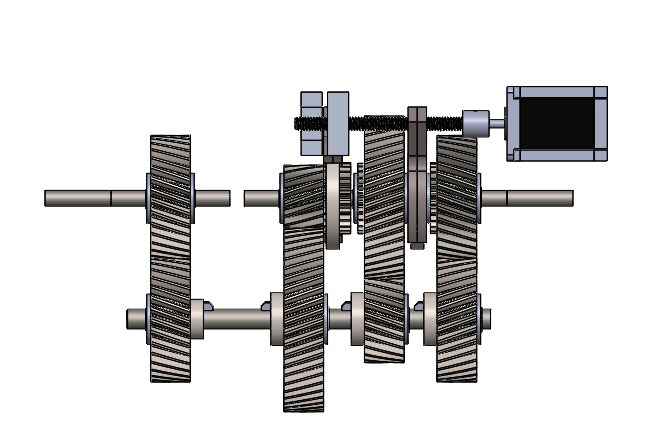
\includegraphics[width =0.7\textwidth]{Cap5_DisenoDetallado/Figuras/Caja_ejes.png}
    \caption{Esquema sistema de transmisión}{Fuente:Elaboración propia}
    \label{fig:Caja_ejes}
\end{figure}

%aqui va la foto que se llama caja ejes
La representación final de el sistema de transmisión, se muestra en la figura \ref{fig:representacion}. 

\begin{figure}[ht!]
    \centering
    \includegraphics[width =0.6\textwidth]{Cap5_DisenoDetallado/Figuras/representación.png}
    \caption{Vista explosionada sistema final}{Fuente:Elaboración propia}
    \label{fig:representacion}
\end{figure}

% aqui va representación

\begin{figure}[ht!]
    \centering
    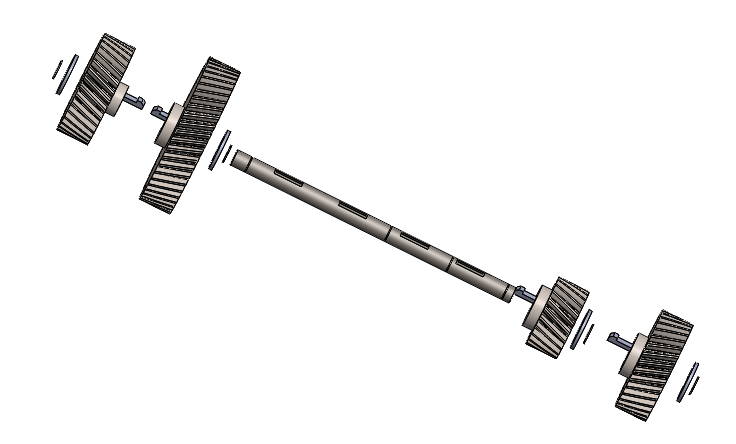
\includegraphics[width =0.8\textwidth]{Cap5_DisenoDetallado/Figuras/eje_intermedio.png}
    \caption{Exploxionado eje intermedio}{Fuente:Elaboración propia}
    \label{fig:eje_inter}
\end{figure}
\begin{figure}[ht!]
    \centering
    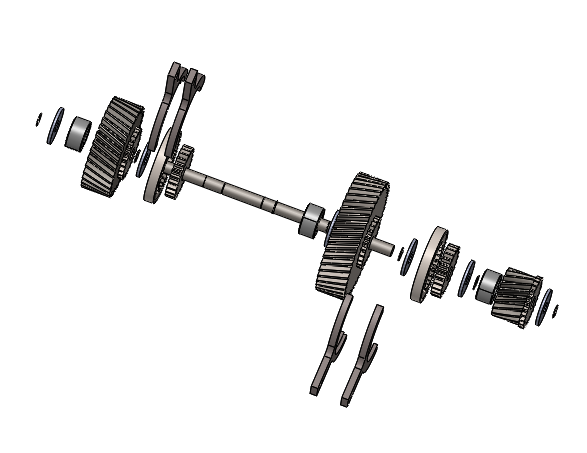
\includegraphics[width =0.8\textwidth]{Cap5_DisenoDetallado/Figuras/eje_de_salida.png}
    \caption{Exploxionado eje de salida}{Fuente:Elaboración propia}
    \label{fig:Eje_salida}
\end{figure}
En la figura \ref{fig:eje_inter} se muestra en mas detalle el eje secundario o intermedio, mientras que en la figura \ref{fig:Eje_salida}, se muestra el eje de salida con los engranajes flotantes.


%eje intermedio

\newpage
~
\newpage

\subsection{Planos}
\begin{figure}[ht!]
    \centering
    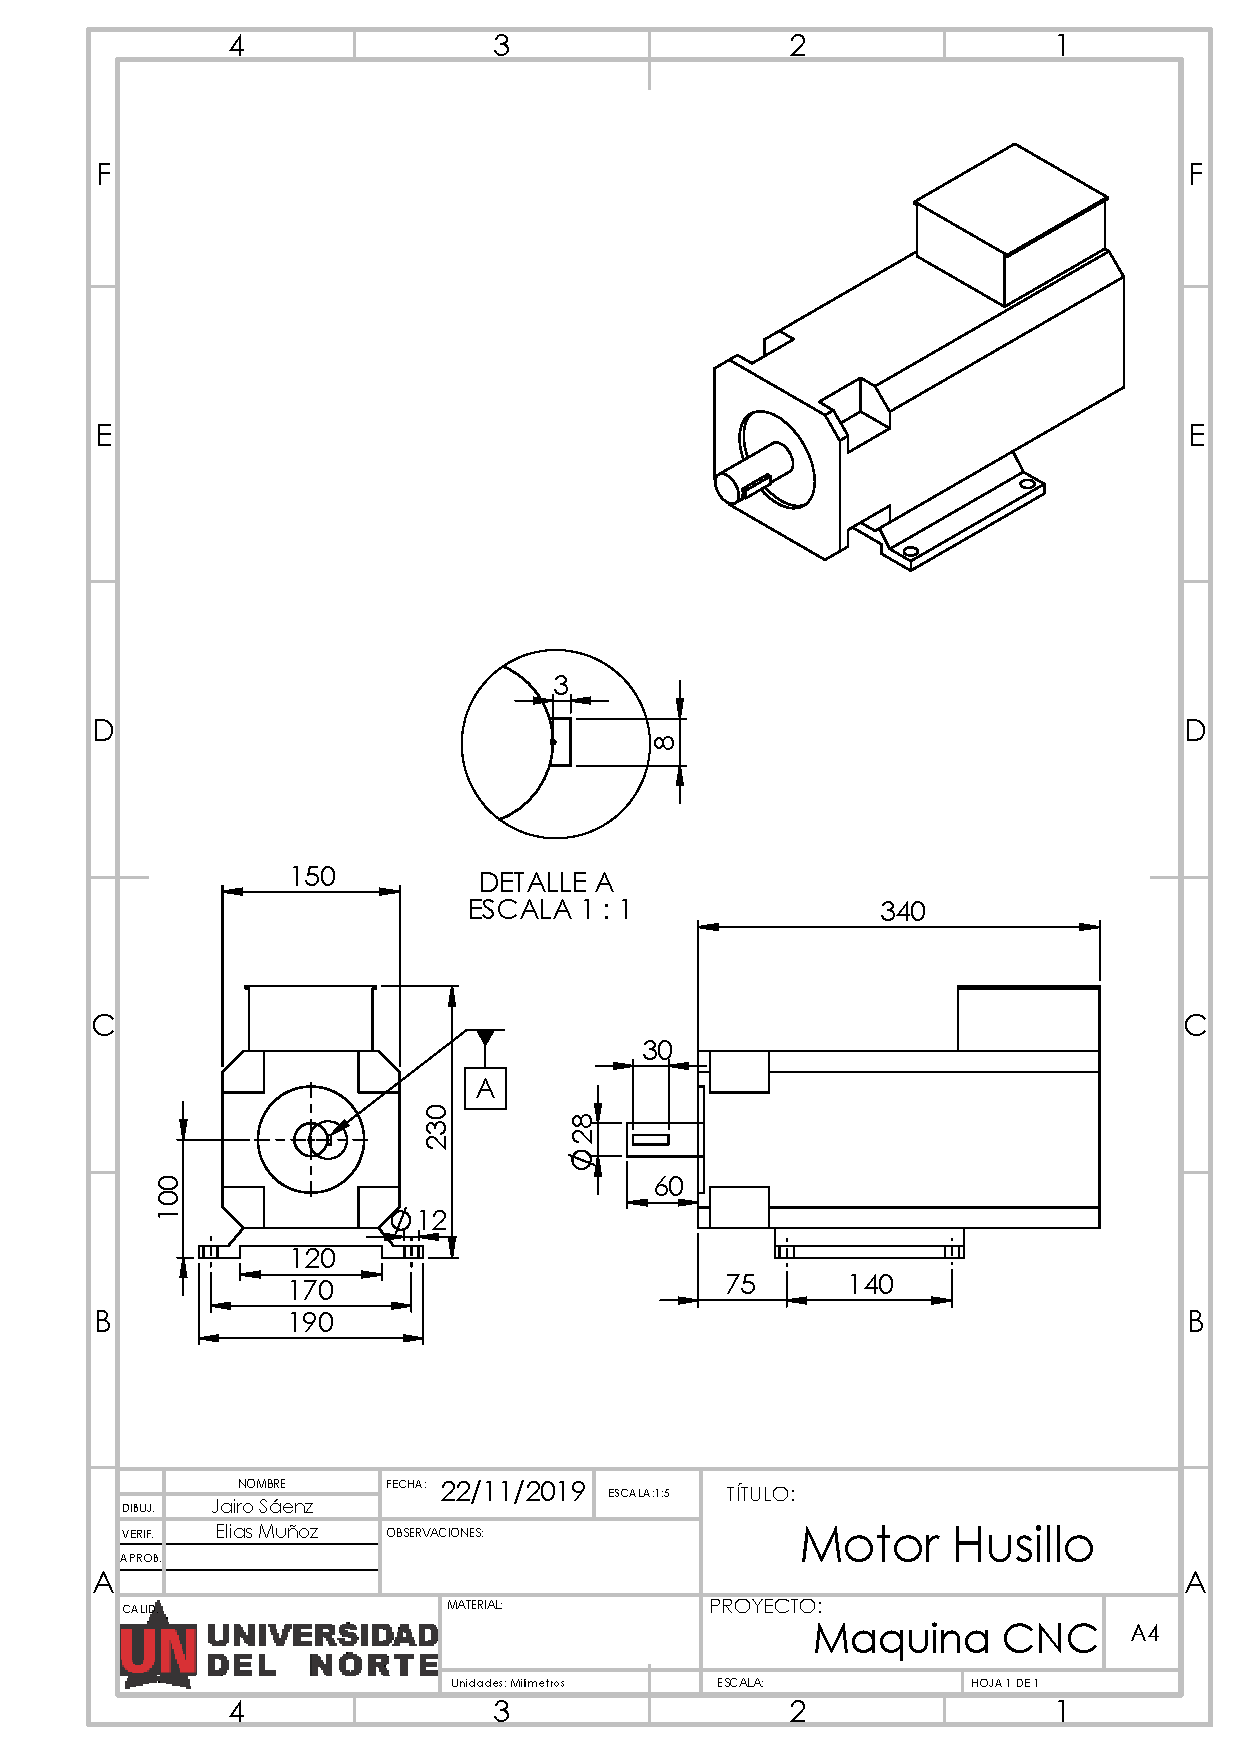
\includegraphics[width =0.8\textwidth]{Cap5_DisenoDetallado/Figuras/motor_electrico.PDF}
    \caption{Plano del Servo motor}{Fuente:Elaboración propia}
    \label{fig:Motor_servo}
\end{figure}
\newpage
\begin{figure}[ht!]
    \centering
    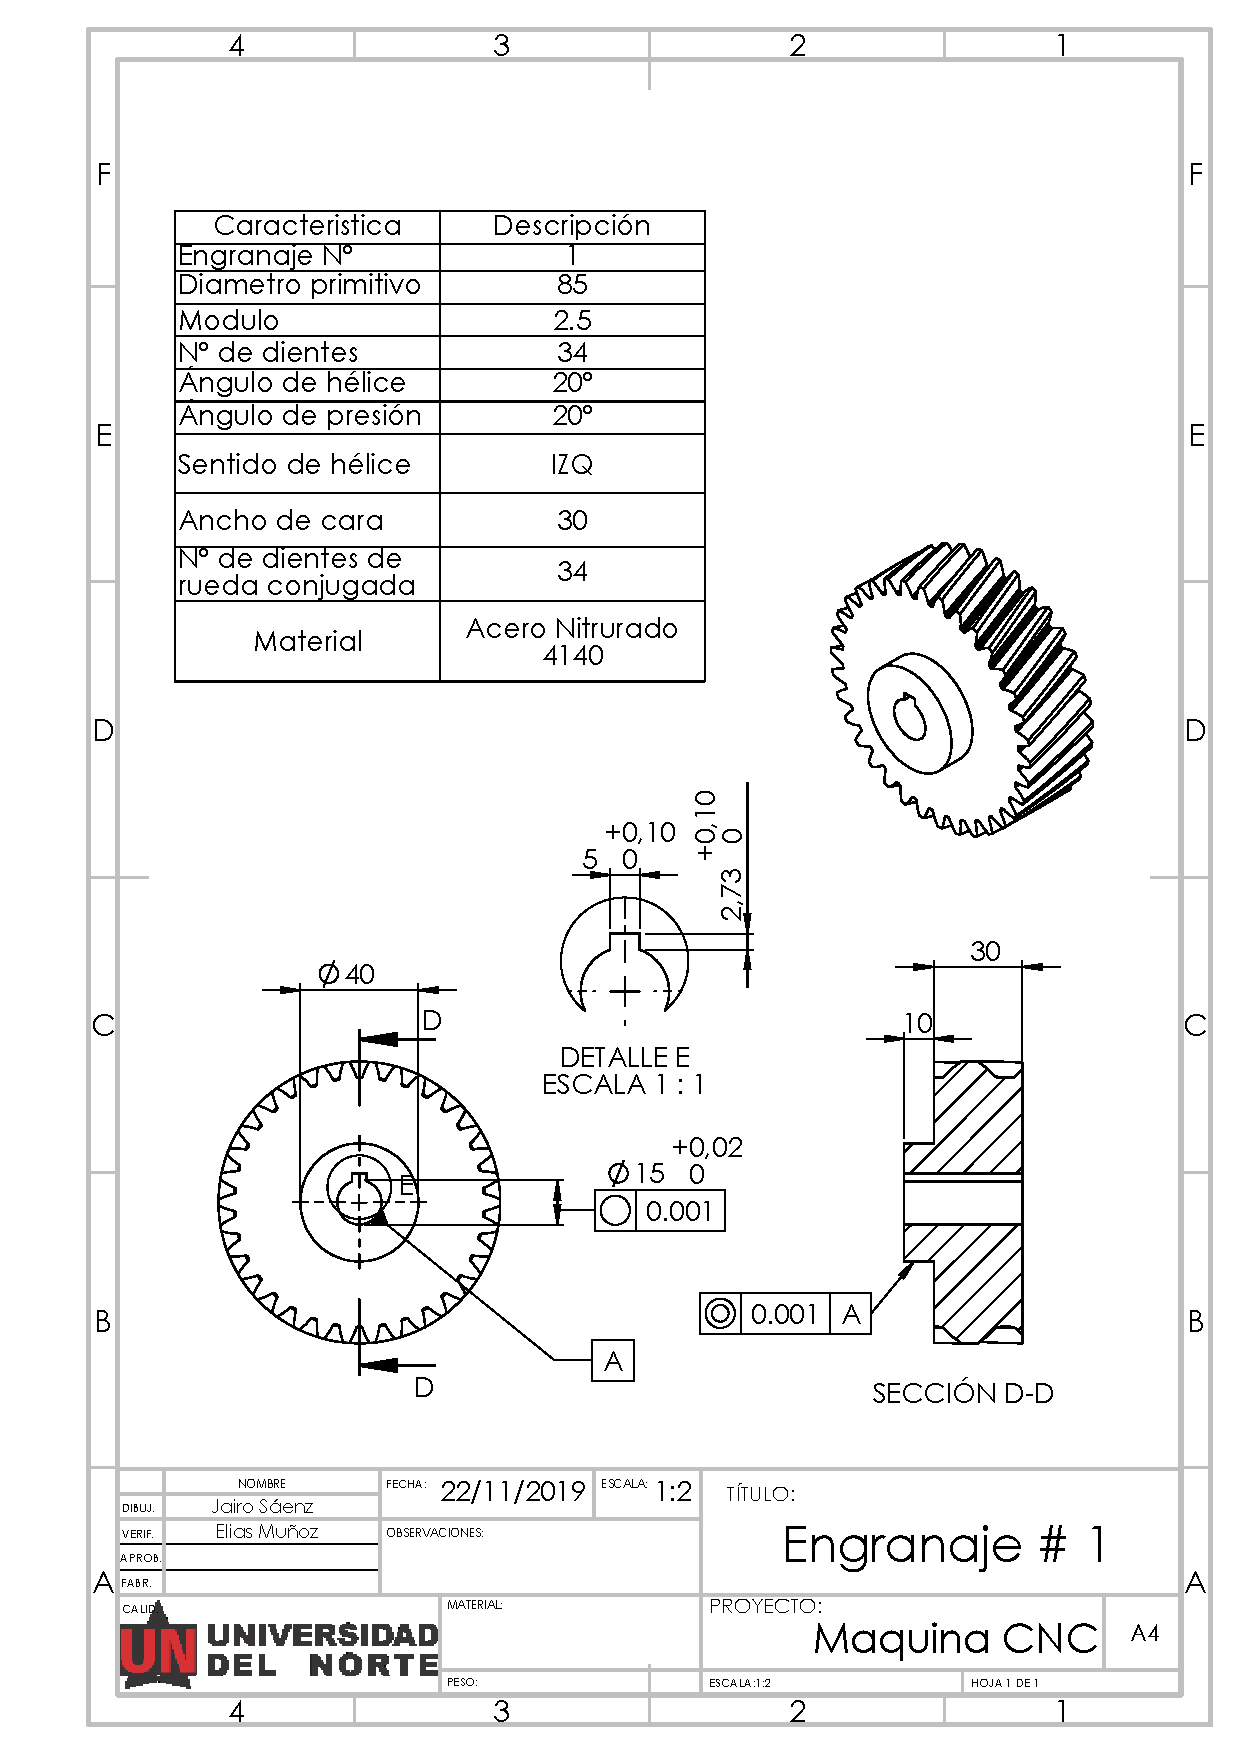
\includegraphics[width =0.8\textwidth]{Cap5_DisenoDetallado/Figuras/engranaje_1.PDF}
    \caption{Plano del engranaje}{Fuente:Elaboración propia}
    \label{fig:Planos_engranaje}
\end{figure}
\newpage
\begin{figure}[ht!]
    \centering
    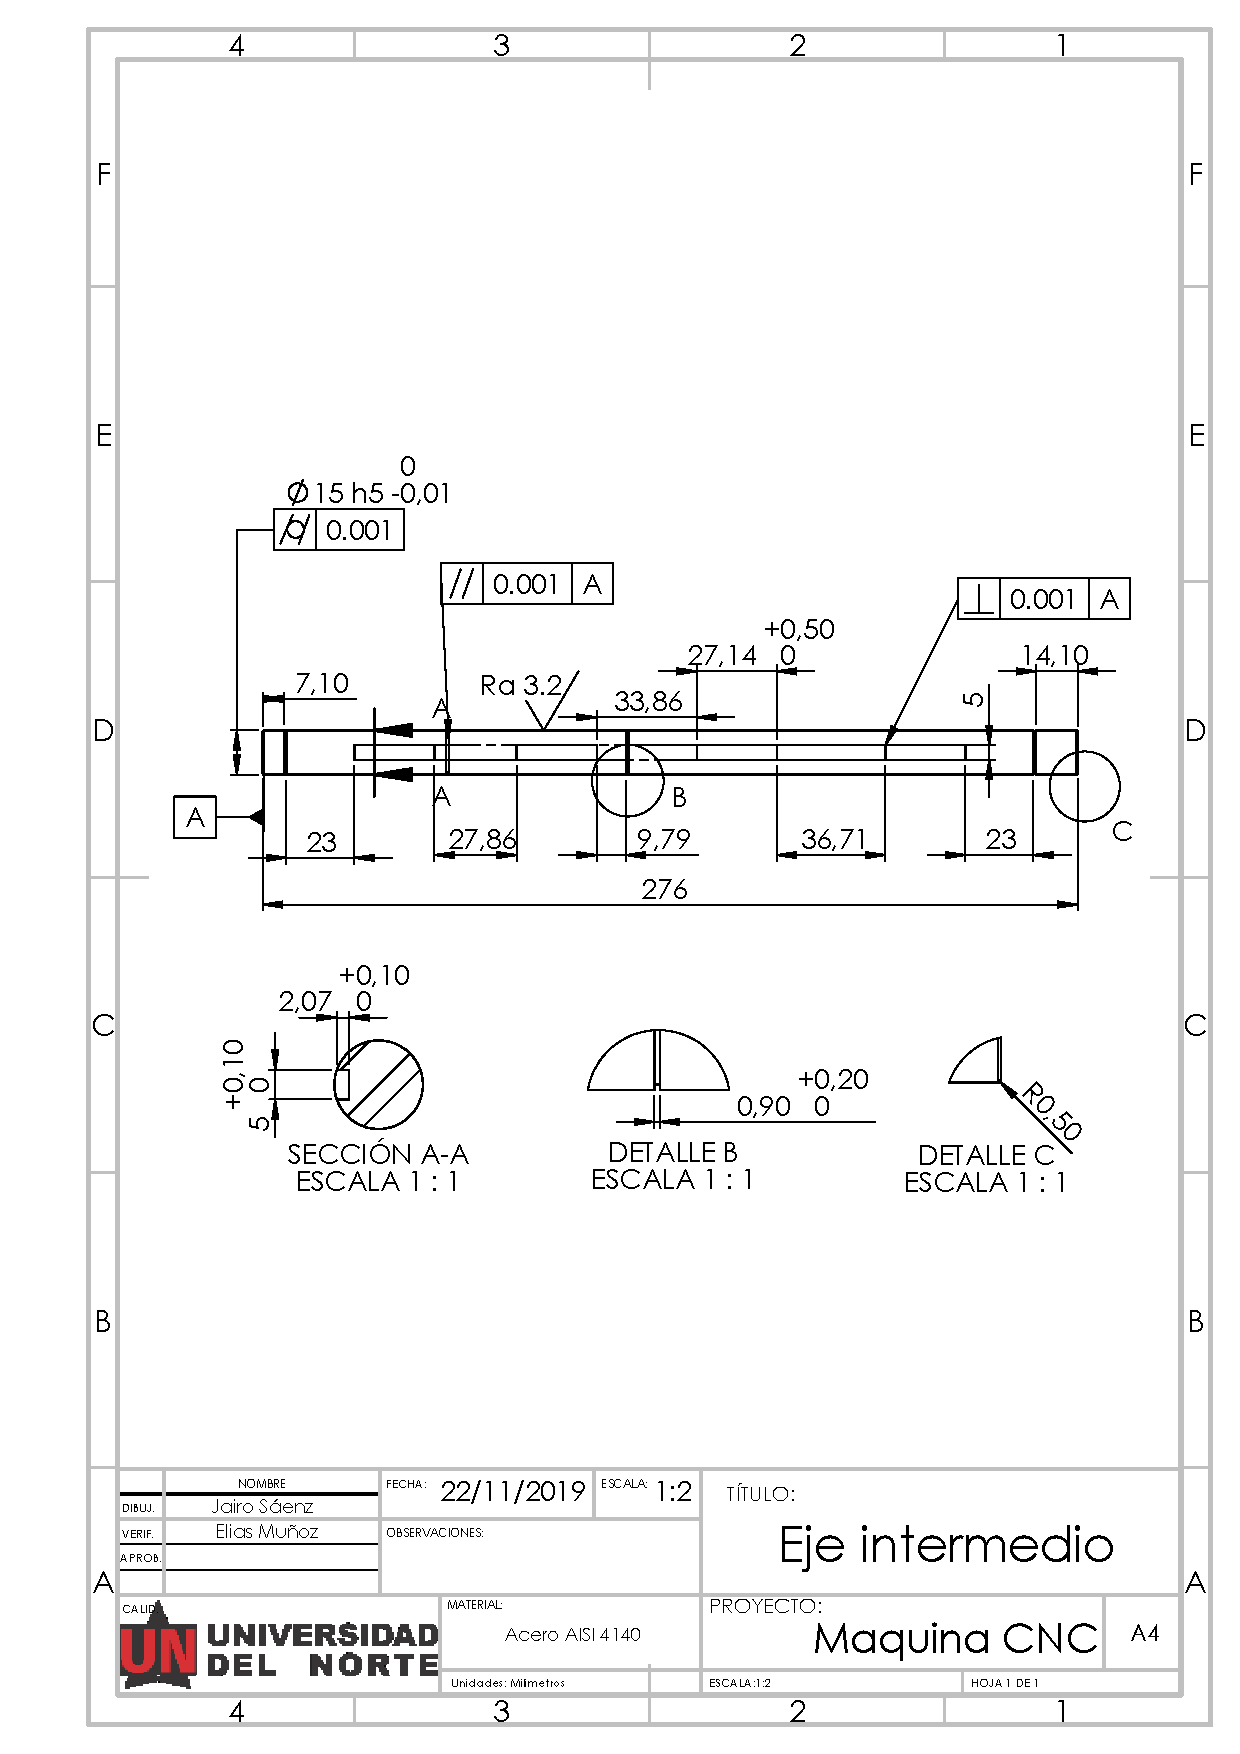
\includegraphics[width =0.8\textwidth]{Cap5_DisenoDetallado/Figuras/eje2.PDF}
    \caption{Plano del eje}{Fuente:Elaboración propia}
    \label{fig:Planos_eje}
\end{figure}
